\documentclass[11pt]{article}
\usepackage{icmlko}
\begin{document}

\title{손잡이 넷 중 처음으로 하나가 살았다 --- 봉우리가 없는 손잡이}
\author{월드모델 실험실}
\date{노트 396 · 2026년 8월 2일}
\maketitle

\begin{abstract}
노트 395가 판 표기값의 씨앗 잡음을 쟀다 --- 자료를 한 글자도 안 바꿔도
SD 0.0033, 폭 0.0121 이다. 그 노트의 남은 것 첫 줄이 ``$K$ 를 올리면
주는가''였다. 배깅 자루가 여덟 개뿐이니 늘리면 줄 것이다.

\textbf{예상보다 빨리 준다.} $K = 8 / 16 / 32$ 에서 씨앗 SD 가
$0.0045 / 0.0027 / \mathbf{0.0010}$ --- $1/\sqrt{K}$ 가 예상하는 2배가
아니라 \textbf{4.5배}다.

\textbf{그런데 판 자체도 오른다} --- $0.4450 / 0.4462 / \mathbf{0.4476}$
으로 단조다. 그러면 이것은 표기 바꿈이 아니라 \textbf{모형 바꿈}이라
관문을 돌려야 한다.

\begin{center}
$K{=}32$ 대 $K{=}8$: 짝 12뽑기 판 $\mathbf{+0.0031}$ · SD 0.0029 ·
\textbf{11/12} · 조건 ② 통과
\end{center}

두 팔 다 씨앗 0 을 썼으니 ``씨앗 0 이 $K{=}8$ 에 나빴을 뿐''일 수 있다.
\textbf{뽑기마다 씨앗도 바꿔 다시 쟀다} --- 같은 $+0.0031$ · 11/12 이고,
이번에는 \textbf{열한 도메인이 전부 양수}다.

\textbf{채택한다. 새 챔피언은 $\mathbf{0.4476 \pm 0.0004}$}(씨앗 6개
평균)이고, 씨앗 SD 가 $0.0033 \to 0.0010$ 으로 준다.

\textbf{이것이 손잡이 넷 중 처음 산 것이다.} 노트 216 이 알파를,
216 · 243 이 $\tau$ 를, 272 가 깊이를 죽였다. 셋 다 \textbf{봉우리가 있는}
편향--분산 손잡이라 안쪽에서 고르면 빗나갔다. $K$ 는 봉우리가 없다 ---
자루를 늘리면 분산만 준다. \textbf{``고르는'' 문제가 아니라 ``얼마나
낼까'' 문제이고, 값은 적합 시간 4배($5.8 \to 24.3$초)다.}
\end{abstract}

\section{왜 이 손잡이는 다른가}

노트 190 · 216 · 272 가 세운 손잡이 규약은 이렇다: 안쪽 분할을 다섯 번
옮겨 보고 봉우리 지수가 0.5 를 넘고 최고가 셋 이상에서 겹쳐야 고른다.
알파 · $\tau$ · 깊이가 다 거기서 떨어졌고, 노트 272 는 ``축이 늘면서
곡면이 평평해졌다''고 적었다.

\textbf{$K$ 는 그 규약이 다루는 종류의 손잡이가 아니다.} 봉우리를 찾는
것이 아니라 \emph{얼마나 살지}를 정하는 값이다 --- 배깅 자루를 늘리면
앙상블 분산이 단조로 줄고, 이론상 최적은 무한대다. 그래서 안쪽 분할로
``고를'' 것이 없고, 대신 \textbf{유보에서 이득이 비용을 넘는지}만 물으면
된다.

그 물음이 관문이다.

\begin{figure}[t]
\centering
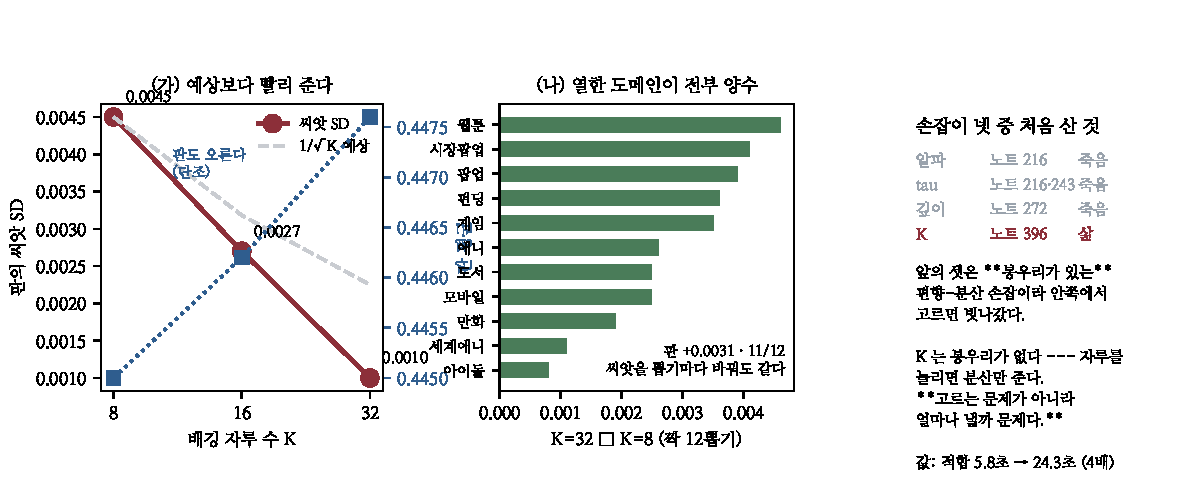
\includegraphics[width=\linewidth]{figs/fig396.pdf}
\caption{\textbf{(가)} $K$ 별 씨앗 SD(붉은)와 판 평균(파란). SD 가
$1/\sqrt{K}$(회색 점선)보다 빨리 준다. \textbf{(나)} $K{=}32$ 대 $K{=}8$
짝 12뽑기의 도메인별 차 --- 전부 양수. \textbf{(다)} 손잡이 넷의 운명.}
\label{fig:main}
\end{figure}

\section{쟀다}

\textbf{잡음.} 챔피언 자료를 고정하고 $K$ 와 씨앗만 바꿔 여섯 번씩 냈다.

\begin{center}
\begin{tabular}{lrrrr}
\hline
$K$ & 적합 초 & 판 평균 & 씨앗 SD & 팝업 SD \\
\hline
8 & 5.8 & 0.4450 & 0.0045 & 0.0357 \\
16 & 11.8 & 0.4462 & 0.0027 & 0.0198 \\
32 & 24.3 & \textbf{0.4476} & \textbf{0.0010} & 0.0140 \\
\hline
\end{tabular}
\end{center}

$1/\sqrt{K}$ 라면 $K{=}32$ 에서 0.0023 이 나와야 하는데 0.0010 이다.
자루를 늘리면 순위 평균이 안정되면서 도메인마다의 흔들림도 같이 주는데,
그 둘이 곱해져 예상보다 빨리 준 것으로 읽는다(관측으로 둔다).

\textbf{관문.} 두 팔에 같은 되뽑기를 주고 12뽑기.

\begin{center}
\begin{tabular}{lrrr}
\hline
 & 판 차 & SD & 부호 \\
\hline
씨앗 고정(둘 다 0) & $+0.0031$ & 0.0029 & 11/12 \\
\textbf{뽑기마다 씨앗도 바꿈} & $+0.0031$ & 0.0024 & \textbf{11/12} \\
\hline
\end{tabular}
\end{center}

\textbf{두 번째가 중요하다.} 첫 관문은 두 팔 다 씨앗 0 이라, 씨앗 0 이
$K{=}8$ 에 유독 나빴다면 이득이 부풀 수 있다. 뽑기마다 씨앗을 바꿔도
같은 값이 나오고 \textbf{열한 도메인이 전부 양수}이므로 그 걱정은 없다
(첫 관문에서는 팝업 $-0.0065$ · 만화 $-0.0002$ 로 둘이 음수였는데, 그것이
씨앗 하나의 우연이었다).

조건 ② 는 두 관문 다 통과다.

\section{값과 대가}

\textbf{얻은 것.} 판 $+0.0031$(11/12) · 씨앗 SD $0.0033 \to 0.0010$ ·
팝업 씨앗 SD $0.0357 \to 0.0140$. 노트 395 가 ``배포 도메인의 표기값이
제일 흔들린다''고 적은 것이 절반 이하로 준다.

\textbf{낸 것.} 적합 한 번이 5.8 초에서 24.3 초로 4배다. 12뽑기 관문
하나가 팔 둘이면 $12 \times 2 \times 24.3 \approx 10$ 분이다. 이번 사이클에
돌린 관문이 열 개가 넘으니 무시할 값은 아니다.

\textbf{그래도 낸다.} 노트 395 가 보였듯 $K{=}8$ 에서는 이번 사이클 채택
넷 중 둘($+0.0012$ · $-0.0015$)이 표기값으로는 잡음에 묻혔다. \textbf{판이
자기 변화를 못 보는 상태였다.}

\section{남은 것}

\begin{center}
\begin{tabular}{lll}
\hline
항목 & 왜 값이 큰가 & 어떻게 \\
\hline
$K{=}64$ 까지 & 32 에서 아직 안 꺾였다 & 같은 관문, 비용 8배 \\
다른 정식화의 $K$ & F18 만 배깅이다 & F6 · F21 에 배깅을 붙여 본다 \\
지난 대장 수 다시 & $K{=}8$ 로 적은 수들이다 & 씨앗 SD 를 옆에 붙인다 \\
애니 나머지 & 덮음 36\% & 수집 중 \\
\hline
\end{tabular}
\end{center}

\end{document}
